\documentclass[a4paper,12pt]{article}
\usepackage{styles/iplouccfg}
\usepackage{styles/zhfontcfg}
\usepackage{styles/iplouclistings}


\title{\LaTeX{}简短使用手册} %标题
\author{孙雪\ 郑海永}  %作者
\date{2013年07月31日} %日期,不加默认为当前日期

\begin{document}

\maketitle
\tableofcontents %目录

\section{基础知识}

\subsection{\LaTeX{}源文件}

\subsubsection{空白距离}

空多个空格 与   一个空格相同;%空多个空格跟一个空格效果相同

空多行


与空一行效果相同  %空多行与空一行效果相同

\subsubsection{特殊字符}

\# \$ \% \^ \& \_ \{ \} %特殊字符

\subsubsection{\LaTeX{}命令}

\TeX{} I 命令后加空格 %命令后加空格

\textsl{斜体} %设置斜体

新的一行 \newline 新的一行

\subsubsection{注释}

短注释 % 短注释
\begin{comment}
balala
\end{comment}   %较长注释采用comment环境

\section{文本排版}

\subsection{断行和分页}

\subsubsection{对齐段落}

另起一行而不是另起一段\\  %另起一行而不是另起一段
在强制断行后还禁止分页\\* %在强制断行后还禁止分页
另起一页\newpage %另起一页

\subsection{内置字符串}

\today 当前日期

\TeX

\LaTeX

\LaTeXe

\subsection{特殊字符和符号}

\subsubsection{引号}

``前引号 \qquad"后引号 \qquad‘’单引号

\subsubsection{破折号和连字号}

daughter-in-law 连字号

pages 13--67 短破折号

yes---or no? 长破折号

$-1$ 减号

\subsubsection{波浪号}

http://rich.edu/$\sim$demo

\subsubsection{度的符号}

$-30\,^{\circ}\mathrm{C}$

\subsubsection{欧元符号}

\texteuro

\subsubsection{省略号}

\ldots

\subsubsection{连字符}

shelf\mbox{}ful  禁止连字符

\subsubsection{注音符号和特殊字符}

H\^otel, na\"\i ve\\
sm\o rrebr\o d, !'Se\ norita!\\
Sch\"onbrunner Schlo\ss{}
Stra\ss e

\subsection{单词间隔}

句号后加大写字母不空格. M

句号后空格加大写字母.M

\subsection{标题、章、节}

\paragraph{段落}
出版的第一步就是作者把打好字的手稿交给出版公司,然后由图书设计者来决定整个文档的布局。图书设计者会把他的排版说明写进作者的手稿里,再交给排版者,由排版者根据这些说明来排版全书。

\subparagraph{子段落}

排版设计是一门工艺。不熟练的作者认为书籍设计仅仅是个美学问题,因而经常会犯严重的格式错误。

\subsection{脚注}
Footnotes\footnote{This is a footnote.} are often used by people using \LaTeX.

\subsection{强调}

\underline{下划线}

\emph{在印刷的书中用斜体字体排印要强调的单词}

\subsection{环境}

\subsubsection{Itemize、Enumerate、Description}

\flushleft
\begin{enumerate} %条目
\item You can mix the list environments \cite{1:article} to your taste:
\begin{itemize}
\item But it might start to look silly.
\item[-] With a dash.
\end{itemize}
\item Therefore remember:
\begin{description}
\item[Stupid] things will not become smart because they are in a list.
\item[Smart] things, though, can be presented beautifully in a list.
\end{description}
\end{enumerate}

\subsubsection{左对齐、右对齐和居中}

\begin{flushleft}
左对齐
\end{flushleft}

\begin{flushright}
左对齐
\end{flushright}

\begin{center}
居中对齐
\end{center}

\subsubsection{引用、语录和韵文}

一个例子:
\begin{quote}
按照顺序阅读这些章节是很重要的这本书毕竟不长。一定要认真阅读例子,因为在贯穿全篇的各种例子里包含了很多的信息。

\end{quote}
例子结束

\subsubsection{摘要}

\begin{abstract}
The abstract
\end{abstract}

\subsubsection{表格}

\begin{table}[!htp] %插表
\label{tab:1}
\centering
\begin{tabular}{|c|c|c|c|}
\hline
0.5&0&0&0\\
\hline
0&1&0&0\\
\hline
0&0.25&0.75&0\\
\hline
0&0&0&1\\
\hline
\end{tabular}  
\caption{一个表格}
\end{table}
通过表\ref{tab:1},我们可以得出\ldots

\subsubsection{图}

\begin{figure}[!htb] %插图
\centering
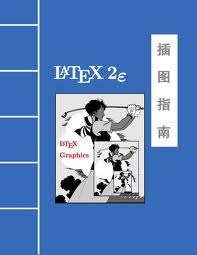
\includegraphics[width=0.5\textwidth]{latex_figure.jpeg}
\caption{\LaTeX{}插图指南}
\label{fig:1}
\end{figure}
通过图\ref{fig:1},我们可以得出\ldots

\subsubsection{参考文献}

BibTeX 模板格式分为好几类:article\cite{1:article}, book\cite{2:book}, misc\cite{3:misc}等等 

\section{数学公式}

\subsection{综述}

\subsubsection{行间式样}

和的平方:$c^{2}=a^{2}+b^{2}$

心型:\begin{math}\heartsuit\end{math}

$\lim_{n \to \infty}\sum_{k=1}^n \frac{1}{k^2} = \frac{\pi^2}{6}$

\subsubsection{显示式样}

求$a$与$b$的和:
\begin{displaymath}a+b=c\end{displaymath}

和的平方:\[c^{2}=a^{2}+b^{2}\]

\begin{displaymath}
\lim_{n \to \infty}
\sum_{k=1}^n \frac{1}{k^2}
= \frac{\pi^2}{6}
\end{displaymath}

\subsubsection{公式编号}

\begin{equation} \label{eq:eps}
\epsilon > 0
\end{equation}
从公式(\ref{eq:eps}), 我们得出\ldots

\subsection{数学模式的群组}

\begin{equation}
a^x+y \neq a^{x+y}
\end{equation}

\subsection{数学公式的基本元素}

\begin{description}
\item[希腊字母]
$\alpha, \beta, \gamma, \Gamma, \Delta, \lambda, \xi, \pi, \mu, \Phi, \Omega$

\item[指数和下标]$a_{1}$, $e^{x^2}\neq {e^x}^2$

\item[平方根] $\sqrt{x}$, $\sqrt[3]{2}$ 

\item[水平线]$\overline{m+n}$, $\underline{m+n}$

\item[水平括号] $\underbrace{a+b+\cdots+z}_{26}$

\item[导数]$y=x^{2}\qquad y’=2x\qquad y’’=2$

\item[乘号]$x_{1}\cdot x_{2}$

\item[log等类的函数名通常用直立字体]
\begin{flushleft}$\arccos, \cos, \csc, \exp, \ker, \limsup,\arcsin, \cosh, \deg, \gcd, \lg, \ln, \arctan$\\$ \cot \det, \hom, \lim, \log,
\arg, \coth, \dim, \inf, \liminf, \max, \sinh, \sup, \tan$\\$ \tanh, \min, \Pr,
\sec, \sin$ 如极限:$\lim_{x \rightarrow 0}\frac{\sin x}{x}=1$
\end{flushleft}

\item[取模函数]$a\bmod b$, $x\equiv a \pmod{b}$

\item[分式]$1\frac{1}{2}$, $\frac{x^2}{k+1}$, $1/2$

\item[二项式系数]$\binom{n}{k},\mathrm{C}_n^k$

\item[符号堆积]$\stackrel{!}{=}$

\item[积分号,累加,累乘]$\int_{0}^{\frac{\pi}{2}} \qquad \sum_{i=1}^{n} \qquad \prod_\epsilon$

\item[括号]
\begin{itemize}
\item 自动调整括号尺寸 
\begin{displaymath}
1 + \left( \frac{1}{ 1-x^{2} }
\right) ^3
\end{displaymath}
\item 指定括号尺寸
$\big(\Big(\bigg(\Bigg($\quad$\big\}\Big\}\bigg\}\Bigg\}$\quad
$\big\|\Big\|\bigg\|\Bigg\|$
\end{itemize}

\item[竖直点列,对角线点列]$\vdots\quad \ddots$
\end{description}

\subsection{垂直取齐}

\begin{displaymath}
\mathbf{X} =
\left( \begin{array}{ccc}
x_{11} & x_{12} & \ldots \\
x_{21} & x_{22} & \ldots \\
\vdots & \vdots & \ddots
\end{array} \right)
\end{displaymath}

\begin{displaymath}
y = \left\{ \begin{array}{ll}
a & \textrm{if $d>c$}\\
b+x & \textrm{in the morning}\\
l & \textrm{all day long}
\end{array} \right.
\end{displaymath}

\begin{displaymath}
\left(\begin{array}{c|c}
1 & 2 \\
\hline
3 & 4
\end{array}\right)
\end{displaymath}

等号取齐:
\begin{eqnarray}
f(x) & = & \cos x
\\
f’(x) & = & -\sin x
\\
\int_{0}^{x} f(y)dy &
= & \sin x
\end{eqnarray}

长等式指定在哪断和如何缩进:
{\setlength\arraycolsep{2pt}
\begin{eqnarray}
\sin x & = & x -\frac{x^{3}}{3!}
+\frac{x^{5}}{5!}-{}
\nonumber\\
&& {}-\frac{x^{7}}{7!}+{}\cdots
\end{eqnarray}}

\begin{eqnarray}
\lefteqn{ \cos x = 1
-\frac{x^{2}}{2!} +{} }
\nonumber\\
& & {}+\frac{x^{4}}{4!}
-\frac{x^{6}}{6!}+{}\cdots
\end{eqnarray}

\subsection{虚位}

${}^{12}_{\phantom{1}6}\textrm{C} \qquad {}^{12}_{6}\textrm{C} $

$\Gamma_{ij}^{\phantom{ij}k} \qquad \Gamma_{ij}^{k} $ 

\subsection{定理、定律}

\newtheorem{law}{Law} %定理
\begin{law}\label{law:t} 
This is my interesting theorem.
\end{law}
通过定理\ref{law:t},我们得出\ldots

\begin{proof}
\[E=mc^2\]
\end{proof}

\subsection{粗体符号}

\begin{displaymath}
\mu, M \qquad
\boldsymbol{\mu}, \boldsymbol{M}
\end{displaymath}

\section{代码高亮}

\subsection{Matlab}

\lstinputlisting{matlab_code.m} %插入Matlab代码({}中为代码地址)

\subsection{python}

\begin{lstlisting}
for i = 1:3
\end{lstlisting}

\begin{python}
#!/usr/local/bin/python
print "Hello World"
os.system("""
VAR=even;
sed -i "s/$VAR/odd/" testfile;
for i in `cat testfile` ;
do echo $i; done;
echo "now the tr command is removing the vowels";
cat testfile |tr 'aeiou' ' '
""") 
\end{python}

\subsection{bash}

\begin{bash}
#!/bin/bash
if [ $# == 1 ]; then
    echo -ne "Deleting FILES including [$1] in the CURRENT directory ...\n\n"
    for i in $(tree -a -f -i | grep "$1")
    do
      echo -ne "Deleting $i\n"
      rm -f $i
    done
elif [ $# == 2 ]; then
    echo -ne "Deleting FILES including [$1] in [$2] directory ...\n"
    for i in $(tree -a -f -i $2 |grep "$1")
    do
      echo -ne "Deleting $i\n"
      rm -f $i
    done    
else
    echo -ne "Arguments Error.\n"
    echo -ne "Usage:\n"
    echo -ne "\t$0 STRING\n"
    echo -ne "\t$0 STRING DIRECTORY\n"
fi
cd ~/
\end{bash}

\subsection{plain}

\begin{plaintext}
user = zhenghaiyong
email = zhenghaiyong@gmail.com
\end{plaintext}


% references
\bibliographystyle{plain}
\bibliography{brief_manual} %参考文献

\end{document}
